Circuit simulation can be performed at different levels of abstraction. 
Behavioral simulation is the highest level of abstraction and functional simulation is the next highest. 
Technically, the only difference between behavioral and functional simulation is the inclusion of unit-delays within the circuit for functional. 
The addition of unit delays for cells in the simulated circuit allows for the comparison of ``theoretical delays'' among different circuits. 
Behavioral or functional simulation is used to used in industry to verify that a circuit is meeting its intended function. 
During functional simulation, functional test patterns are supplied to a circuit, and circuit output responses are monitored to ensure that the circuit is functioning as intended. 
This can be done in several different ways, but the goal is to supply meaningful inputs to the circuit, and observe meaningful outputs. 


Consider any generic processor.
If the processor receives an instruction that does not contain a valid op-code, it will be put into an unknown op-code state. 
In order to test this processor for defects, we would like to supply it with instructions that test all of the internal circuitry. 
Supplying it with one unknown opcode would test certain parts of the exception handling routines, but we shouldn't supply the processor with \textit{only} instructions that have unknown opcodes.
If we did, we would not be able to effectively test the rest of the circuitry. 
Supplying a circuit with many different inputs to test all of the corner cases of the state space is the goal of proper functional verification. 


Consider Figure \ref{fig:sd1}. 
This diagram represents the state space of a fabricated circuit. 
We call $S$ the set of all possible ``Circuit goodstates.''
The size of the $S$ is equivalent to $2^{m}$, where $m$ is the number of memory elements the circuit.  
Assume there are three known functions of the circuit: $A, B,$ and $C$. 
These functions are known to use subsets of the states in $S$, denoted by $S_{A}, S_{B},$ and $S_{C}$ respectively.
During manufacture a defect was introduced to the circuit. 
This defect can only be detected if the circuit is operating in a state in goodstate grouping denoted $F$.


\begin{figure}[h!]
\centering
\caption{Arbitrary State Space\label{fig:sd1}}
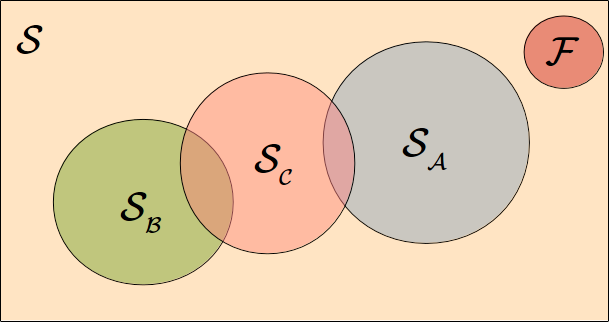
\includegraphics[scale=0.5]{Figures/sd1.png}
\end{figure} 

Fortunately, this fault does not conflict with any of the three known functions state spaces.
Imagine that a customer was only going to use functions $A, B,$ and $C$.
They would never experience the fault, because they never operate the circuit in a state space that overlaps with it. 
This means that there would be absolutely no reason to discard this circuit, because it would still be useful to the customer. 
By performing this sort of functional simulation of circuits, we can rate faults in terms of how many times they might be encountered during functional use.
Using functional simulation as well as a few additional parameters to rate these faults in terms of their general importance allows  more efficient resource allocation. 
This resource allocation is the primary purpose of this research. 